\subsection{Simulazioni Monte-Carlo}

L'obiettivo di questa sezione è l'introduzione di delle tecniche Monte-Carlo che consentano di simulare un modello di Ising mono-dimensionale con 
numero di costituenti finito e che presenti condizioni periodiche al contorno, in modo tale che gli spin posti agli estremi della catena 
interagiscano fra loro come primi vicini. Dato che in questo modo tutti gli spin sono equivalenti fra loro ed il sistema è invariante per 
traslazioni, stiamo in pratica simulando un sistema infinito, con un conseguente netto miglioramento della qualità dei risultati. 
Dopo aver definito una condizione iniziale, che solitamente sono quella a temperatura nulla, con tutti gli spin allineati, oppure 
quella a temperatura infinita caratterizzata da momenti magentici orientati casualmente, il primo passo è quello di generare una 
nuova configurazione tentando di invertire uno spin. La differenza in energia fra lo stato di partenza e quello di arrivo determina 
la probabilità d'accettazione della mossa, dato che per l'\textit{algoritmo di Metropolis} \cite{M(RT)2} si ha che 

\begin{equation}
    A\left(\nu\,|\,\mu\right)\,=\,\text{min}\left[1,\,e^{-\beta\left(E_{\nu}\,-\,E_{\mu}\right)}\right]
    \label{eq: Metropolis_1D}
\end{equation}

Chiaramente se la configurazione $\nu$ ha energia inferiore di quella $\mu$, la mossa viene sempre accettata. In caso contrario, è 
possibile che lo spin non venga invertito ed il nuovo elemento della catena di Markov generata dall'algoritmo di Metropolis è identico 
a quello precedente. In seguito è possibile osservare l'implementazione di tale algoritmo in Nim: lo stesso calcolo viene eseguito 
nuovamente ad ogni iterazione, scegliendo lo spin di cui provare il flip in modo casuale.



\subsubsection{Generatore di numeri casuali}

Dato che i metodi Monte-Carlo sono una classe di algoritmi numerici che sfruttano i numeri pseudo-casuali, è auspicabile lavorare 
con un generatore dotato di un lungo periodo (i numeri generati non si ripetono spesso) e che sia efficiente, in modo da ridurre le 
tempistiche computazionali. Le simulazioni che hanno portato ai risultati presenti in questa dispensa sono state effettuate con un 
generatore della famiglia PCG \cite{pcg2014}, di cui è riportata l'implementazione



\begin{minted}[frame=lines, fontsize=\small, bgcolor=blue!10]{nim}
type 
    PCG* = tuple[state, incr: uint64] ##\
    ## The `PCG` type represents the state of a Permuted Congruential 
    ## Generator (PCG), a family of simple fast space-efficient statistically 
    ## good algorithms for random number generation.

    RandomSetUp* = tuple[inState, inSeq: uint64] ##\
    ## The `RandomSetUp` type is used to initialize a `PCG` generator.


proc random*(gen: var PCG): uint64 =
    ## Get a random uint64 from a `PCG`.

    var 
        oldstate = gen.state
        xorshift = uint32(((oldstate shr 18) xor oldstate) shr 27)
        rot = int32(oldstate shr 59)

    gen.state = oldstate * uint64(6364136223846793005) + gen.incr
    result = ((xorshift shr rot) or (xorshift shl ((-rot) and 31)))


proc newRandomSetUp*(rg: var PCG): RandomSetUp {.inline.} = 
    ## Create a new `RandomSetUp` from a `PCG`.
    (rg.random, rg.random)


proc newPCG*(setUp: RandomSetUp): PCG = 
    ## Create a new `PCG` with the given `RandomSetUp`.

    (result.state, result.incr) = (0.uint64, (setUp.inSeq shl 1) or 1)
    discard result.random
    result.state += setUp.inState
    discard result.random


proc rand*(pcg: var PCG): float32 =
    ## Get a random float32 uniformly distributed over the interval (0, 1)
    pcg.random.float32 / 0xffffffff.float32

proc rand*(pcg: var PCG; a, b: float32): float32 =
    ## Get a random float32 uniformly distributed over the interval (a, b)
    a + pcg.rand * (b - a)
\end{minted}    

I numeri pseudo-casuali vengono generati lavorando con interi senza segno, che consentono di fare operazioni fra bit molto efficienti. 
La corretta implementazione è stata testata imponendo un particolare RandomSetUp e valutando la sequenza generata. Sebbene l'implementazione 
del PCG sia riportata nella sezione relativa al modello di Ising mono-dimensionale, tale algoritmo è stato utilizzato anche per l'Ising 2D.



\subsubsection{Termalizzazione}

Una simulazione Monte-Carlo è detta all'equilibrio nel momento in cui viene correttamente campionato il peso statistico di Boltzmann 
$p\left(\mu\right)$. Se il sistema viene inizializzato in uno dei due stati presentati in precedenza, ossia quello a temperatura 
nulla (con spin paralleli) oppure a $T$ infinita (con spin orientati casualmente up oppure down) e si vuole performare una simulazione a 
temperatura finita, sarà necessario del tempo computazionale prima che venga raggiunto l'equilibrio, poichè sara necessario accettare 
alcune mosse.

Un modo qualitativo per valutare la durata della termalizzazione consiste nel graficare una quantità d'interesse, 
come può essere la magnetizzazione oppure l'energia interna del sistema. Tali osservabili presenteranno una fase di transitorio 
iniziale in cui il sistema si scorrela dalla condizione iniziale, per poi fluttuare attorno ad un valore pressochè costante. Non è 
sempre garantito che si raggiunga l'equilibrio, in quanto è possibile rimanere bloccati in uno stato metastabile per tempistiche 
computazionali relativamente lunghe. Per evitare di valutare in maniera errata la durata della fase di termalizzazione è consigliabile 
eseguire lo stesso processo per diverse condizioni iniziali e per diversi seed del generatore di numeri casuali, in modo da considerare 
diverse traiettorie nello spazio delle fasi.  




\subsubsection{Misure e Data-Blocking}

Una volta che il sistema ha raggiunto l'equilibrio, è possibile misurare le osservabili d'interesse senza che i valori d'aspettazione 
siano influenzati dalla fase di transitorio. Per valutare la durata minima della simulazione che consenta di ottenere delle stime 
statisticamente significative è necessaria una misura del tempo di correlazione $t_c$, che esplicita quale sia il numero di mosse 
da effettuare per passare fa uno stato ad un secondo significativamente differente da quello di partenza. Il modo migliore per 
calcolare $t_c$ consiste nello sfruttare la funzione di autocorrelazione temporale, definita per la magnetizzazione come 

\begin{equation}
    \chi\left(t\right)\,=\,\frac{\left<m\left(t'\right)m\left(t'\,+\,t\right)\right>_{t'}\,-\,\left<m\right>^2}{\sigma^2_m}
    \label{eq: auto_corr_m}
\end{equation}

L'autocorrelazione solitamente presenta una caduta esponenziale con tempo caratteristico pari a quello di correlazione

\begin{equation}
    \chi\left(t\right)\,\sim\,e^{-t/t_c}.
    \label{eq: auto_corr_cad_exp}
\end{equation}

Se si considerano due campioni presi ad un $t_c$ di distanza, la funzione di autocorrelazione assume in presenza di un tale 
intervallo temporale un valore di $1/e$, ancora particolarmente significativo. Se si vuole lavorare con quantità realmente indipendenti 
è necessario campionare a $t\,>\,t_c$; solitamente si impone $t\,=\,t_c$ in modo che il numero di misure significative in una 
simulazione di durata $t_{max}$ è pari a 

\begin{equation}
    n\,=\,\frac{t_{max}}{2 t_c}.
    \label{eq: num_ind_samp}
\end{equation}

Per evitare bias nel campionamento e per ottenere dei valori d'aspettazione adeguati è possibile utilizzare la tecnica del 
data-blocking. Le misure delle osservabili di interesse effettuate durante la simulazione, a distanze temporali del tempo di correlazione, 
vengono divise in gruppi, per ciascuno dei quali viene calcolato il valor medio. La dispersione di questi valori medi fornisce una 
stima dell'errore associato alla grandezza calcolata. In Figura \ref{fig: data_block_tech} è presentata visivamente la tecnica del data-
blocking. Le quantità $g_i$ sono le medie di ciascun gruppo.

\begin{figure}[H]
    \centering
    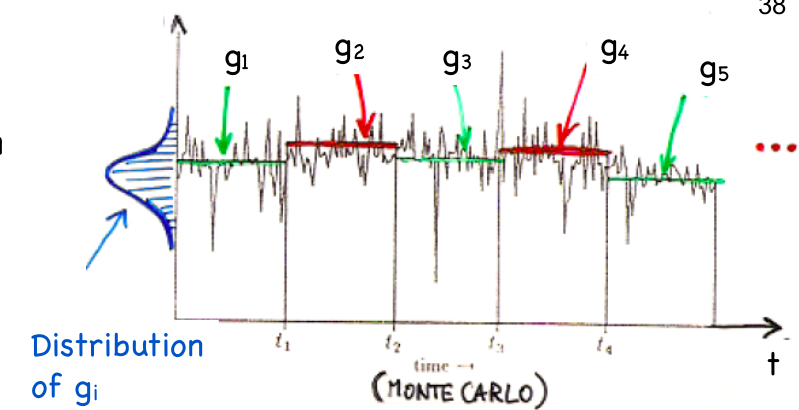
\includegraphics[width=0.6\textwidth]{Immagini/data_blocking.png}
    \caption{Esempio di applicazione della tecnica del data-blocking. Immagine da \cite{galliLSN}.}
    \label{fig: data_block_tech}
\end{figure}

Per determinare quale sia la lunghezza dei blocchi tale da garantire che le medie siano statisticamente indipendenti, si può 
sfruttare il teorema del limite centrale. Nel momento in cui si aumenta la lunghezza dei blocchi, l'errore calcolabile come 

\begin{equation}
    \sigma_{\left<g\right>}\,=\,\sqrt{\frac{1}{N-1}\left(\left<g^2\right>\,-\,\left<g\right>^2\right)}
    \label{eq: error_data_block}
\end{equation}

tende a quello puramente statistico (poichè si va a perdere la correlazione fra le stime) e dopo una certa lunghezza $L$ dei blocchi 
non aumenta più, ma satura ad un valore costante. La lunghezza di saturazione è la minima accettabile per produrre delle stime adeguate. 
Chiaramente maggiore è il numero di blocchi (ossia più lunga è la simulazione), migliore sarà la stima finale della osservabile 
d'interesse.